\section{Dicas Úteis}

Abaixo, seguem algumas dicas que auxiliarão na escrita das seções anteriores.

\subsection{Como referenciar estudos/trabalhos neste documento}

Os principais modos de referenciar estudos/trabalhos são:
\begin{enumerate}[label=\roman*., itemsep=0pt, leftmargin=2.5cm]
    \item Em geral, o autor da obra deve ser citado entre parênteses pelo sobrenome, separado por vírgula da data de publicação. Desse modo, para esse estilo de citação, use o comando \verb|\cite{label_bib}|, onde \texttt{label\_bib} é o rótulo único de uma determinada referência contida no arquivo \texttt{referencias.bib}. Por exemplo:
        \begin{itemize}
            \item \verb|\cite{Russell2003}| $\rightarrow$ \cite{Russell2003}.
        \end{itemize}
    \item Se o nome do autor estiver citado no texto, indica-se apenas a data entre parênteses. Logo, use o comando \verb|\citeonline{label_bib}|. Por exemplo:
        \begin{itemize}
            \item \verb|\citeonline{Wazlawick2021}| $\rightarrow$ \citeonline{Wazlawick2021}.
        \end{itemize}
\end{enumerate}

\subsection{Uso de âncoras (\textit{cross-references}) no texto}

Para referenciar um determinado elemento (seção, tabela, imagem, quadro, etc.) no texto, é necessário marcar tal elemento com um rótulo. Para isso, use o comando \verb|\label{rotulo}|. Desse modo, o nome desse rótulo (\texttt{rotulo}) será útil posteriormente para referenciar esse elemento.

Por fim, para referenciar um elemento, use o comando \verb|\ref{rotulo}|, informando seu rótulo entre as chaves do comando.

\subsection{Exemplos de Imagens, Tabelas, Quadros, Listagem de Código e Algoritmos}

\begin{figure}[!h]
    \centering
    \caption{Exemplo de figura}\label{fig:exemplo_figura}
    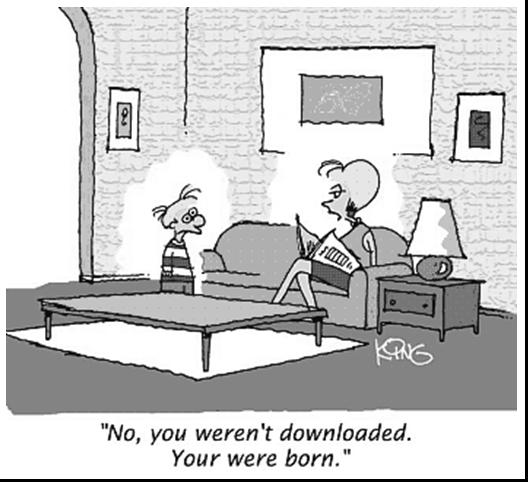
\includegraphics[width=.4\textwidth]{conteudo/figs/fig1.jpg}
    \fonte{\citeonline{SBC2024}}
\end{figure}

\begin{table}[!h]
    \centering
    \caption{Exemplo de Tabela}\label{tb:exemplo_tabela}
    \begin{tabular}{cccc}
        \hline Página & Topo & Baixo & Esquerda/Direita \\\hline
        Primeira & 3,5 & 2,5 & 1,5 \\
        Demais & 2,5 & 2,5 & 1,5 \\ \hline
    \end{tabular}
    \vspace{0.1cm}
    \fonte{Autoria própria (2024)}
\end{table}

\newpage

\begin{quadro}[!h]
    \centering
    \caption{Exemplo de Quadro}\label{tb:exemplo_quadro}
    \begin{tabular}{|c|c|c|c|}
        \hline Página & Topo & Baixo & Esquerda/Direita \\\hline
        Primeira & 3,5 & 2,5 & 1,5 \\ \hline
        Demais & 2,5 & 2,5 & 1,5 \\ \hline
    \end{tabular}
    \vspace{0.1cm}
    \fonte{Autoria própria (2024)}
    \vspace{0.1cm}
    \nota{Lorem ipsum dolor sit amet, consectetur adipiscing elit. Aenean ac viverra urna. Pellentesque vulputate erat vitae suscipit finibus. Vestibulum efficitur turpis vitae tincidunt cursus.}
\end{quadro}

\begin{codigo}[!h]
    \centering
    \caption{Exemplo de Código Fonte em Java}\label{cod:exemplo}
\begin{lstlisting}[language=Java]
public class Exemplo{
    public static void main(String[] args){
        System.out.println("Hello World!");
    }
}
\end{lstlisting}
    \fonte{Autoria própria (2024)}
\end{codigo}

\begin{algoritmo}[!h]
    \centering
    \caption{Método de Ordenação \textit{Bubble Sort}}\label{alg:exemplo}
    \begin{algorithm}[H]
        \SetAlgoBlockMarkers{início}{fim}
        \Dados{$vetor$, conjunto de dados a ser ordenado.}
        \Resultado{$vetor$, conjunto de dados ordenados após a execução do método.}
        \SetKwProg{Fn}{Função}{}{}\SetKwFunction{MetodoBolha}{metodoBolha}
        \SetKwFunction{TamanhoVetor}{obterTamanho}
        \AlgoDisplayBlockMarkers
    	\Fn{\MetodoBolha{vetor}}{
            \Para{inteiro i = 1 \Ate \TamanhoVetor{vetor} - 1}{
                \Para{inteiro j = 1 \Ate \TamanhoVetor{vetor} - i}{
                    \Se{vetor[j] $>$ vetor[j + 1]}{
                        inteiro temp = vetor[j] \\
                        vetor[j] = vetor[j + 1] \\
                        vetor[j + 1] = temp \\
                    }
                }
            }
            \Retorna{vetor}
    	}
    \end{algorithm}
    \fonte{Autoria própria (2024)}
\end{algoritmo}

\newpage